\section{Experiment}
\label{sec:experiment}

\subsection{Dataset and Features}
\label{sec:dataset}

% experiment protocol: Nested cross-validation with Monte-Carlo cross-validation for the inner loop
We experiment methods developed in Section~\ref{sec:trajrec} on trajectories extracted from Flickr photos~\cite{thomee2016yfcc100m}.
The statistics of datasets are shown in Table~\ref{tab:data} and 
the histograms of the number of ground truths for queries are shown in Figure~\ref{fig:hist}.

% dataset stats
\begin{table}[t]
\caption{Statistics of trajectory dataset}
\label{tab:data}
\centering
\setlength{\tabcolsep}{4pt} % tweak the space between columns
\small
\begin{tabular}{l*{5}{r}} \hline
\textbf{Dataset} & \textbf{\#Photos} & \textbf{\#Visits} & \textbf{\#Traj.} & \textbf{\#Users} & \textbf{\#Queries} \\ \hline
Glasgow & 29,019 & 11,434 & 2,227 & 601 & 64 \\
Osaka & 392,420 & 7,747 & 1,115 & 450 & 47 \\
\hline
\end{tabular}
\end{table}


% histogram of #ground truth
\begin{figure}[t]
	\centering
	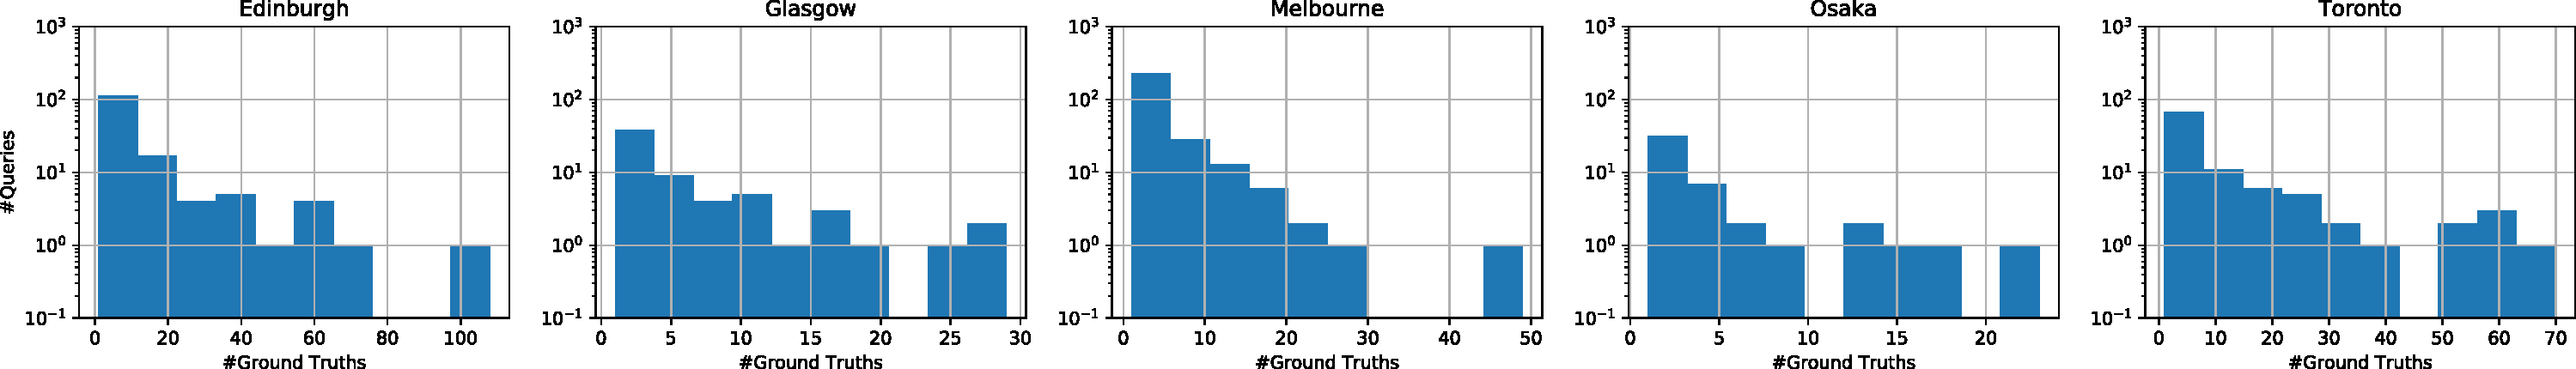
\includegraphics[width=\columnwidth]{hist.pdf}
	\caption{Histogram of the number of ground truth}
	\label{fig:hist}
\end{figure}


% leave-one-out evaluation (with query aggregation)
As described in Section~\ref{sec:queryagg}, 
we first group trajectories according to queries that they conform to,
then evaluate the performance of each algorithm using leave-one-out cross validation,
where we hold each query and its associated trajectories for test and all other trajectories for training.
% model selection (Monte Carlo CV) (with query aggregation): 90/10 random split for 5 times
Furthermore, 
the hyper-parameter (regularisation constant $C$) is tuned using the Monte Carlo cross validation~\cite{burman1989comparative} on training set.

% evaluation metric: kendall's Tau (mention F1, pF1)
To evaluate the performance of each algorithm variant, 
we compute the Kendall's $\tau$ (version $b$)~\cite{kendall1945,agresti2010analysis} to measure the quality of recommendation.
In particular,
we define the rank of POIs $\mathcal{P}$ given trajectory $\mathbf{y} = (y_1,\dots,y_K)$ as
\begin{align*} 
r_\mathbf{y} &= (r_1,\dots,r_j,\dots,r_{|\mathcal{P}|}), \\
r_j &= \sum_{k=1}^K (| \mathcal{P} | - k + 1)  \llb p_j = y_k \rrb, ~ j = 1, \dots, | \mathcal{P} |.
\end{align*}
Unlike the F$_1$ sore on points~\cite{ijcai15} or the F$_1$ score on pairs~\cite{cikm16paper}, 
which only cares about either the set of correctly recommended POIs or the set of correctly predicted POI pairs,
this metric taking both factors into account.

In addition, we take the maximum of all pairs,
i.e.,
\begin{equation*}
\tau_b^{(i)} = 
\max_{(\mathbf{y}, \hat{\mathbf{y}}) \in \{\mathbf{y}^{(ij)}\}_{j=1}^{N_i} \times \{\hat{\mathbf{y}}^{(ij)}\}_{j=1}^k} 
\tau_b(r_\mathbf{y}, r_{\hat{\mathbf{y}}}),
\end{equation*}
where $\{\mathbf{y}^{(ij)}\}_{j=1}^{N_i}$ are the ground truths for query $\mathbf{x}^{(i)}$ and
$\{\hat{\mathbf{y}}^{(ij)}\}_{j=1}^k$ are the top-$k$ recommendations.



\subsection{Experimental Results}
\label{sec:result}

% !TEX root = ./main.tex

\begin{table*}[t]
\caption{Experimental results on trajectory recommendation datasets. The top three rows are baselines, and the bottom four are the methods proposed in this paper. Bolded entries correspond to the best performing method for each metric; italicised entries to the next best method. Higher scores are better.}
\label{tab:result}
\centering
%\setlength{\tabcolsep}{3pt} % tweak the space between columns
\small
\begin{tabular}{l|cc|cc|cc} \hline
                    & \multicolumn{2}{|c}{\textbf{Kendall's $\tau$}}
                    & \multicolumn{2}{|c}{\textbf{F$_1$ score on points}}
                    & \multicolumn{2}{|c}{\textbf{F$_1$ score on pairs}} \\ \cline{2-7}
                    & Osaka & Glasgow 
                    & Osaka & Glasgow  
                    & Osaka & Glasgow \\ \hline
\textsc{Random}     & $0.403\pm0.025$ & $0.410\pm0.032$  
                    & $0.430\pm0.021$ & $0.451\pm0.027$  
                    & $0.057\pm0.024$ & $0.136\pm0.037$ \\
\textsc{Popularity} & $0.567\pm0.034$ & $0.646\pm0.035$  
                    & $0.601\pm0.031$ & $0.681\pm0.032$  
                    & $0.277\pm0.051$ & $0.416\pm0.050$ \\
\textsc{PoiRank}    & $0.646\pm0.040$ & $0.736\pm0.030$  
                    & $0.678\pm0.037$ & $0.764\pm0.027$  
                    & $0.425\pm0.058$ & $0.550\pm0.047$ \\
\midrule
\textsc{SP}         & $0.796\pm0.037$ & $0.865\pm0.027$  
                    & $0.817\pm0.034$ & $0.878\pm0.024$  
                    & $0.665\pm0.055$ & $0.772\pm0.040$ \\
\textsc{SPpath}     & $0.794\pm0.035$ & $0.740\pm0.034$  
                    & $0.814\pm0.032$ & $0.764\pm0.030$  
                    & $0.653\pm0.054$ & $0.591\pm0.047$ \\
\textsc{SR}         & $\mathbf{0.814\pm0.034}$ & $\mathit{0.870\pm0.025}$  
                    & $\mathbf{0.832\pm0.031}$ & $\mathit{0.887\pm0.022}$ 
                    & $\mathit{0.673\pm0.053}$ & $\mathit{0.774\pm0.039}$ \\
\textsc{SRpath}     & $\mathit{0.805\pm0.036}$ & $\mathbf{0.877\pm0.025}$ 
                    & $\mathit{0.821\pm0.033}$ & $\mathbf{0.893\pm0.021}$ 
                    & $\mathbf{0.682\pm0.054}$ & $\mathbf{0.792\pm0.038}$ \\ \hline
\end{tabular}
\end{table*}


% experimental results
The performance of three baselines and four variants based on structured prediction on two datasets are shown in Table~\ref{tab:result}.
The \textsc{Random} baseline simply keep recommending a POI sampled uniformly at random from the whole set of POIs (without replacement),
until we get all the specified number of POIs.
On the other hand, \textsc{Popularity} is slightly smarter which considers the popularity of each POI, 
and recommend the top-$k$ most popular places.
\textsc{PoiRank}~\cite{cikm16paper} is a generalisation of \textsc{Popularity} which consider a number of POI features in addition to its popularity.

We can see from the empirical results that all variants of structured prediction achieve very good performance.
In particular, \textsc{SR} always performs better than \textsc{SP}, 
which suggests that explicitly modelling multiple ground truths helps recommendation.

Furthermore, we observed that sub-tour elimination in training improves the ordering of recommended trajectories, 
as indicated by the F$_1$ score on pairs, 
however, this advantage will not take effect if the multiple ground truths is not modelled explicitly,
which further enforces its importance.
